\subsection{Muon system}

\label{sec:muon}


The di-muon decay channel of the A$^\prime$ has the advantage of a greatly reduced electromagnetic background.  In this case, the only particle background in a muon counter would come from upstream photoproduction of $\pi^+$ and $\pi^-$ pairs that are not fully stopped in the ECal or absorber.  A muon detector will match geometrical acceptances of the tracker and ECal, and will be about a cubic meter in size. With such geometrical coverage, efficiency of detecting high mass A$^\prime$s in $\mu^+\mu^-$ decay channel will be higher than for $e^+e^-$ decays, see Figure \ref{fig:muacc}. Expected low background and high efficiency, the di-muon final state is an attractive complement to A$^\prime$ search using $e^+e^-$ final state, and will add substantial territory in the mass and coupling space. With muon system, HPS will be the only experiment proposed to date to search for heavy photons in an alternative to $e^+e^-$ decay mode.

\begin{figure*}[!ht]
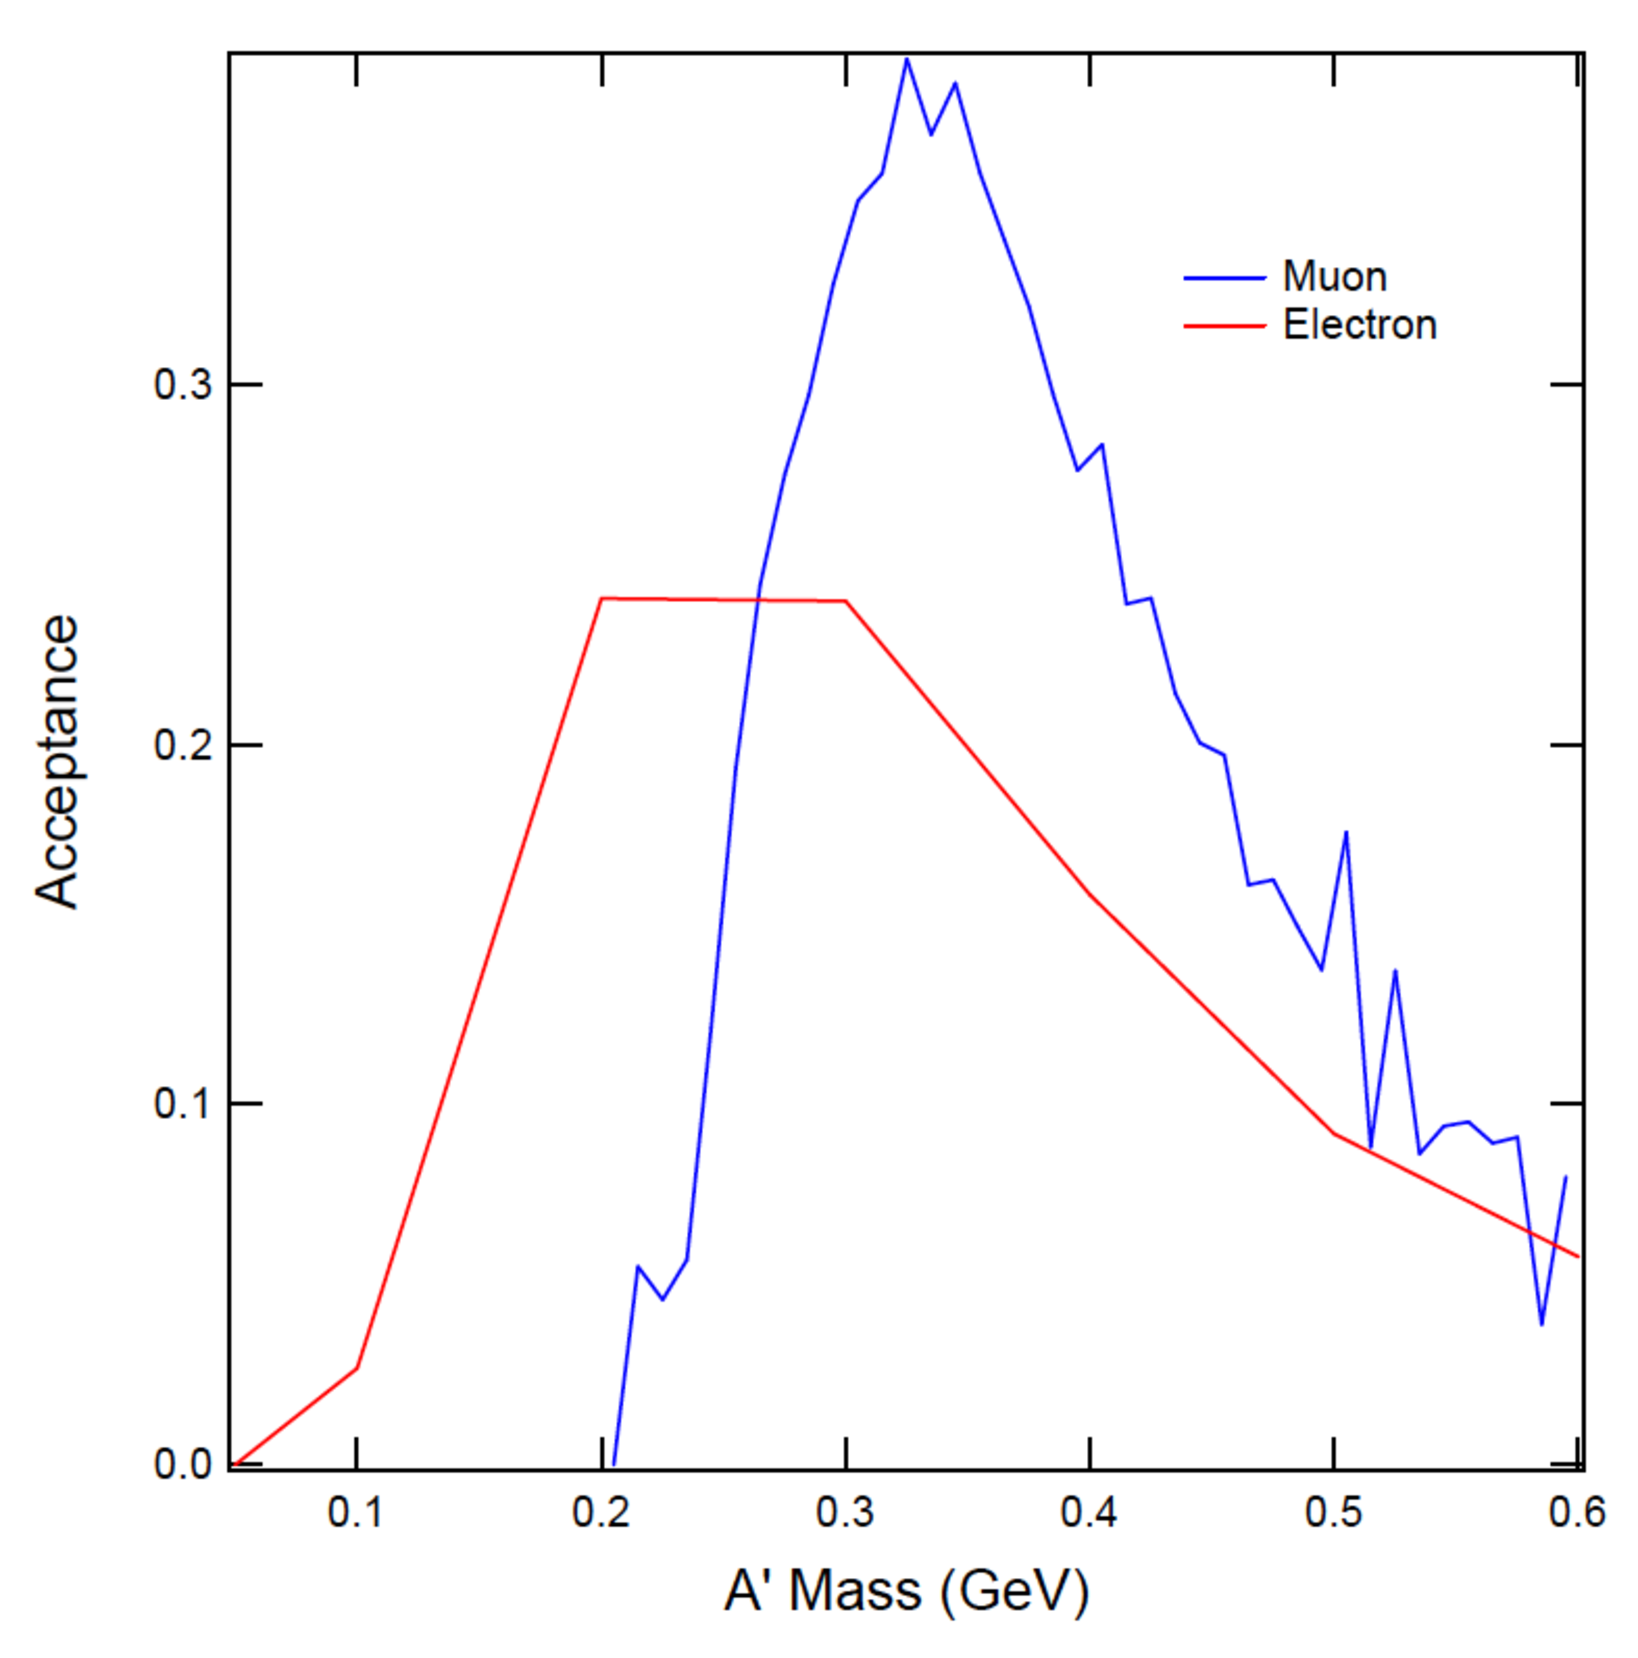
\includegraphics[scale=0.4]{muon/acc.pdf}
\caption{\small{A$^\prime$ detection efficiency through $\mu^+\mu^-$ (blue) and $e^+e^-$ (red) decay channels as a function of mass for 6.6 GeV beam energy.}}\label{fig:muacc}
\end{figure*}

The muon system can easily be constructed with layers of scintillator hodoscopes sandwiched between iron absorbers, and can be added downstream from the rest of the HPS apparatus.
The number of layers and the thickness of absorbers is defined by the $\pi/\mu$ rejection factor. The schematic design of the muon detector was optimized using the GEANT-3 model for the ECal with added layers of iron and scintillators.  In the simulation, muons and pions in the momentum range of $1$ to $4$ GeV/c first passed through the 16 cm of lead tungstate in the ECal and then entered a muon counter with various total absorber thicknesses (see \cite{HPS_PROP} for details).  Detection efficiencies for pions ($\epsilon_\pi$) and muons ($\epsilon_\mu$) were then calculated as a function of absorber thickness and particle momentum.  For low-energy particles ($< 1.7$ GeV) detection in all four layers of scintillator hodoscopes was not considered. Depending on the momentum, particles were not traced behind the third, fourth or fifth absorber.  
Figure \ref{fig:pmrej} shows the resulting rejection factor $\epsilon_\pi/\epsilon_\mu$.  The right-hand plot shows the dependence of  $\epsilon_\pi/\epsilon_\mu$ on the total thickness of the iron absorber, with the best rejection at about 75 cm.  The right-hand plot shows $\epsilon_\pi/\epsilon_\mu$ for a 75 cm absorber as a function of muon momentum.  The suppression of individual pions by two orders of magnitude will suppress pion pairs by 4 orders of magnitude.  

\begin{figure*}[!ht]
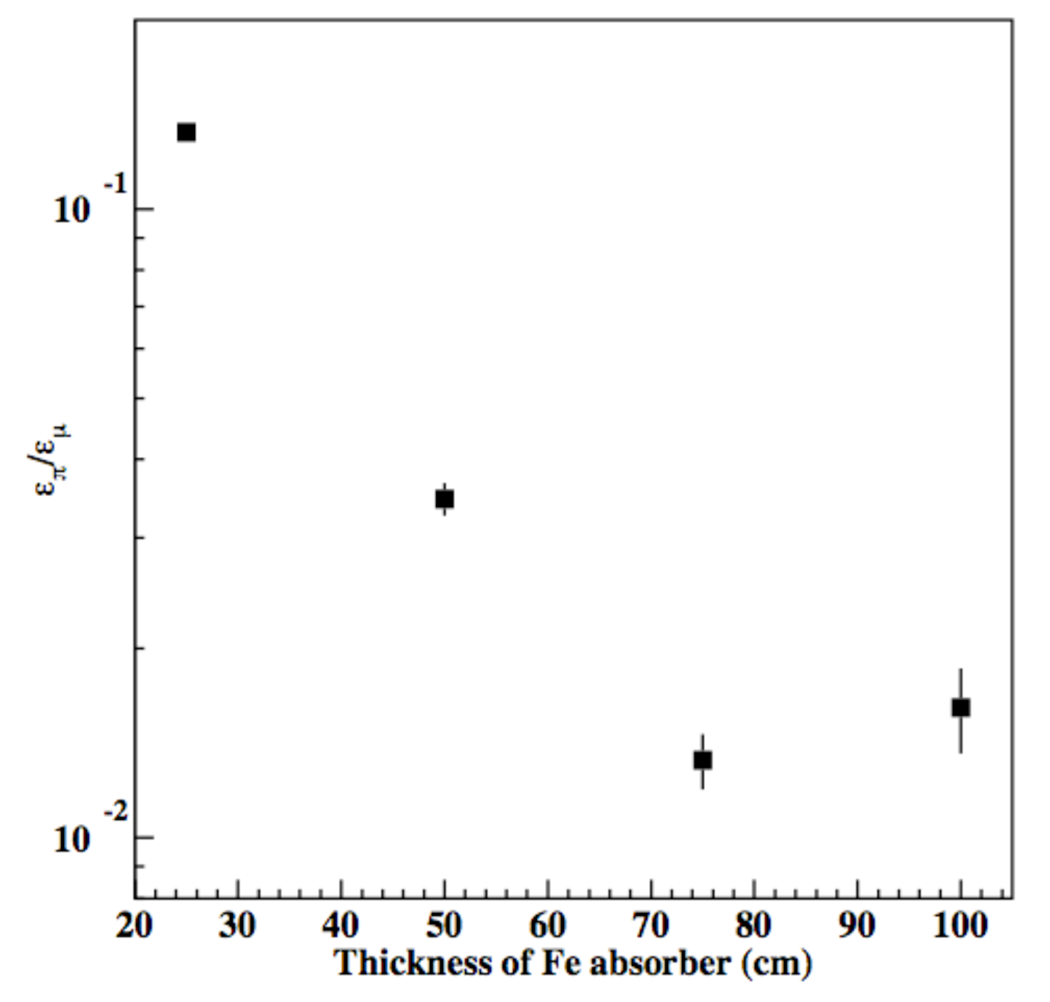
\includegraphics[scale=0.44]{muon/pmrej.pdf}
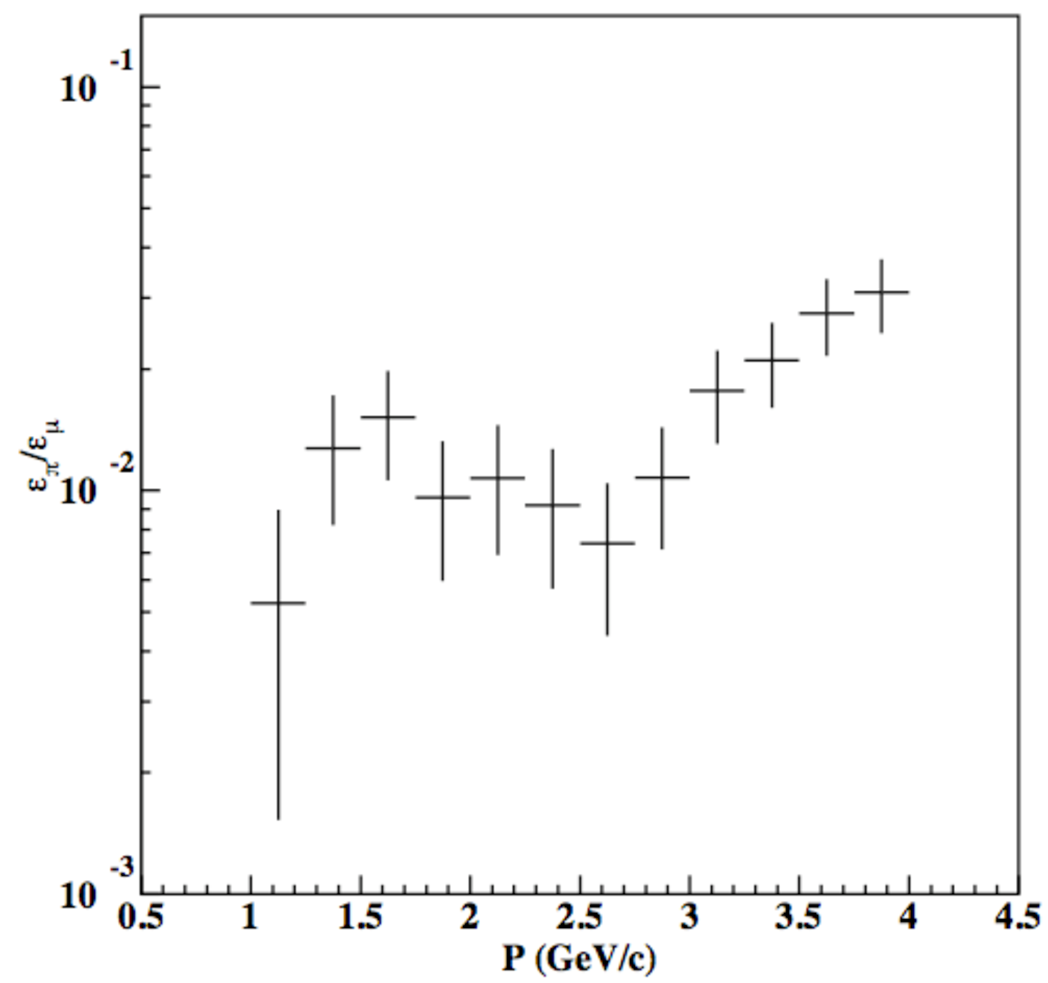
\includegraphics[scale=0.44]{muon/pmrej4.pdf}
\caption{\small{Pion-muon rejection factor $\epsilon_\pi/\epsilon_\mu$ versus total iron absorber thickness
(left) and versus particle momentum for a 75 cm absorber (right).}}\label{fig:pmrej}
\end{figure*}


\subsubsection{Conceptual Design}

On the basis of these simulations, we have designed a muon detector composed of four iron absorbers (total length of $30+15+15+15=75$ cm) with a double-layer scintillator hodoscope positioned after each absorber. The muon detector will be mounted behind the ECal.  The front face of the first absorber will be at $\sim 180$ cm from the target. Similar to the Ecal, the muon detector will consist of two halves, one above and one below the beam.  This segmentation is necessary in order to
minimize the effects of the ``sheet-of-flame" that multitude of low-energy particles in the horizontal plane, swept into the detector acceptance by the dipole analyzing magnet.
The vertical gap between the first hodoscope layers of the two halves is about $5$ cm. Dimensions of hodoscopes and absorbers are shown in Table \ref{tb:muon}.  Figure \ref{fig:HPS_view2} shows a CAD
drawing of the HPS detector, with the muon system on the right, which includes the 4 absorbers (gray), the vacuum box (light gray) between the upper and lower sections, and the final set of scintillator paddles (red). The ECal is directly upstream from the muon detector, with its crystals shown in yellow.  In front of the ECal is a large gray vacuum flange.  The silicon tracker is represented by red and gray rectangles and  the red point on the left is the target position.  

\begin{table}[htdp]
\caption{Dimensions (in cm) of muon system scintillation hodoscopes (H) and iron absorbers (A). }
\begin{center}
\begin{tabular}{|c|c|c|c|c|}
\hline
&H1&H2&H3&H4\\
\hline
Distance from target& 212&232&252&272\\
Width&112&125&138.5&152\\
Hight&10.5&11.5&12.5&13.5\\
\hline
\end{tabular}

\begin{tabular}{|c|c|c|c|c|}
\hline
&A1&A2&A3&A4\\
\hline
Distance from target& 207&227&247&267\\
Width&108.5&122&135&148.5\\
Hight&10&11&12&13\\
Thickness & 30 & 15& 15 & 15\\
\hline
\end{tabular}
\end{center}
\label{tb:muon}
\end{table}%


\begin{figure*}[!ht]
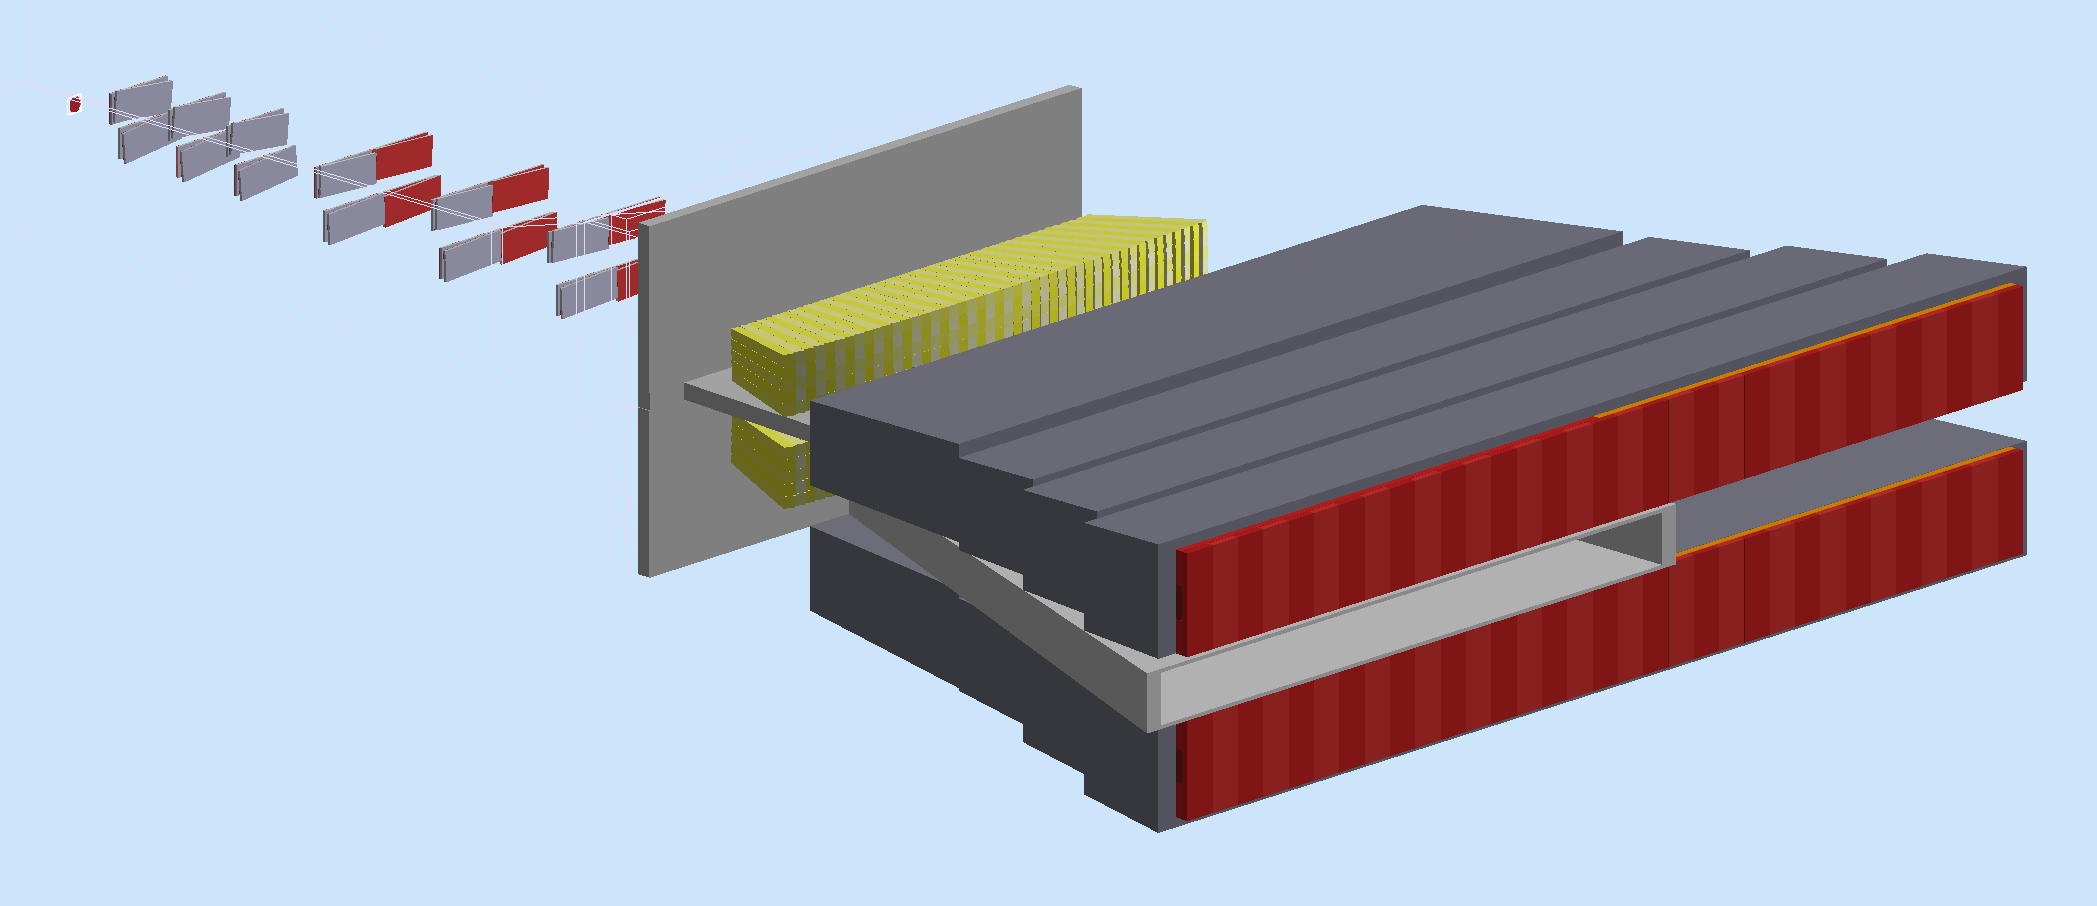
\includegraphics[scale=0.22]{muon/HPS_view2.png}
\caption{\small{CAD drawing of the HPS detector setup.  From left to right this consists of the target (red dot), the silicon tracker
(gray and red rectangles), the large shielding wall (gray), the ECal lead tungstate crystals (yellow, two shades), the muon counter absorbers
(gray), and the final muon counter scintillators (red, two shades).}}
\label{fig:HPS_view2}
\end{figure*}

%\begin{figure*}[!ht]
%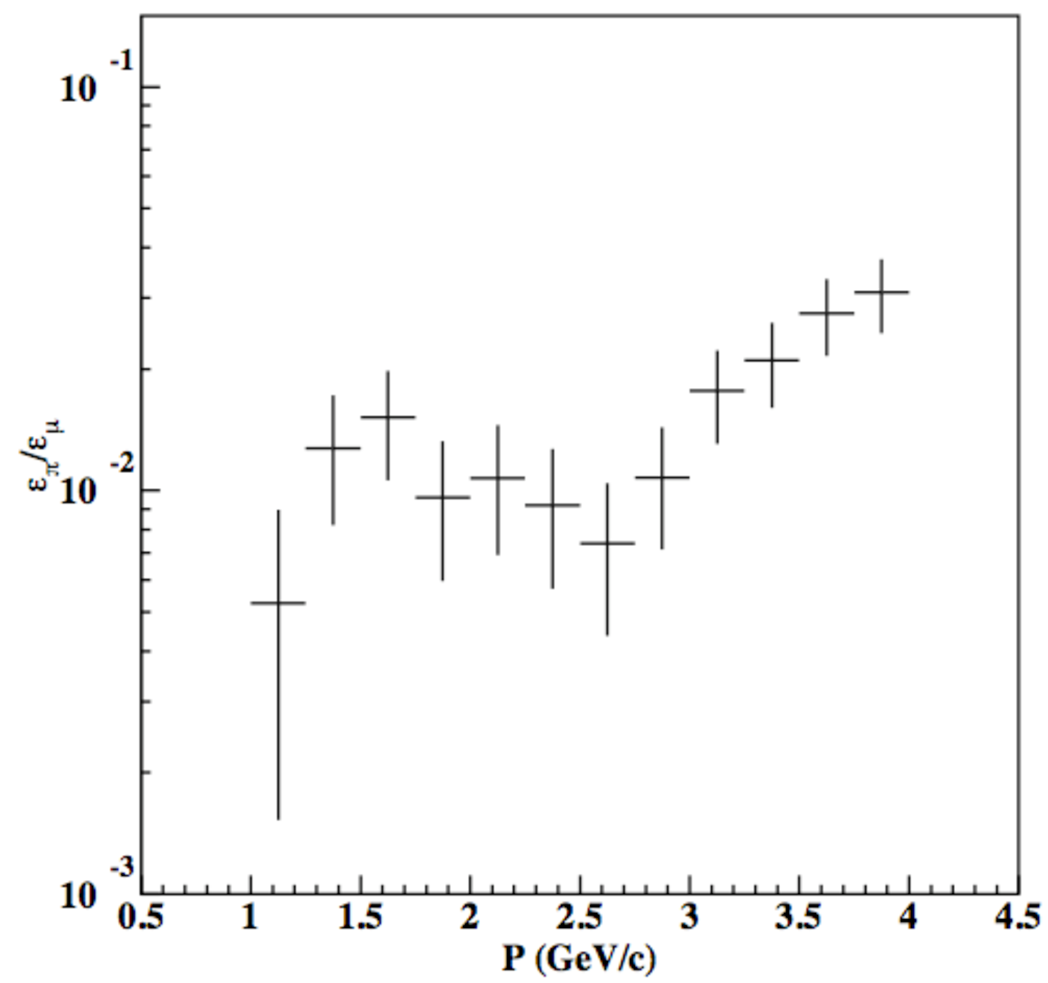
\includegraphics[scale=0.8]{muon/pmrej4.pdf}
%\caption{\small{Pion-muon rejection factor as a function of the iron absorber thickness.}}\label{fig:pmrejp}
%\end{figure*}

\begin{figure*}[!ht]
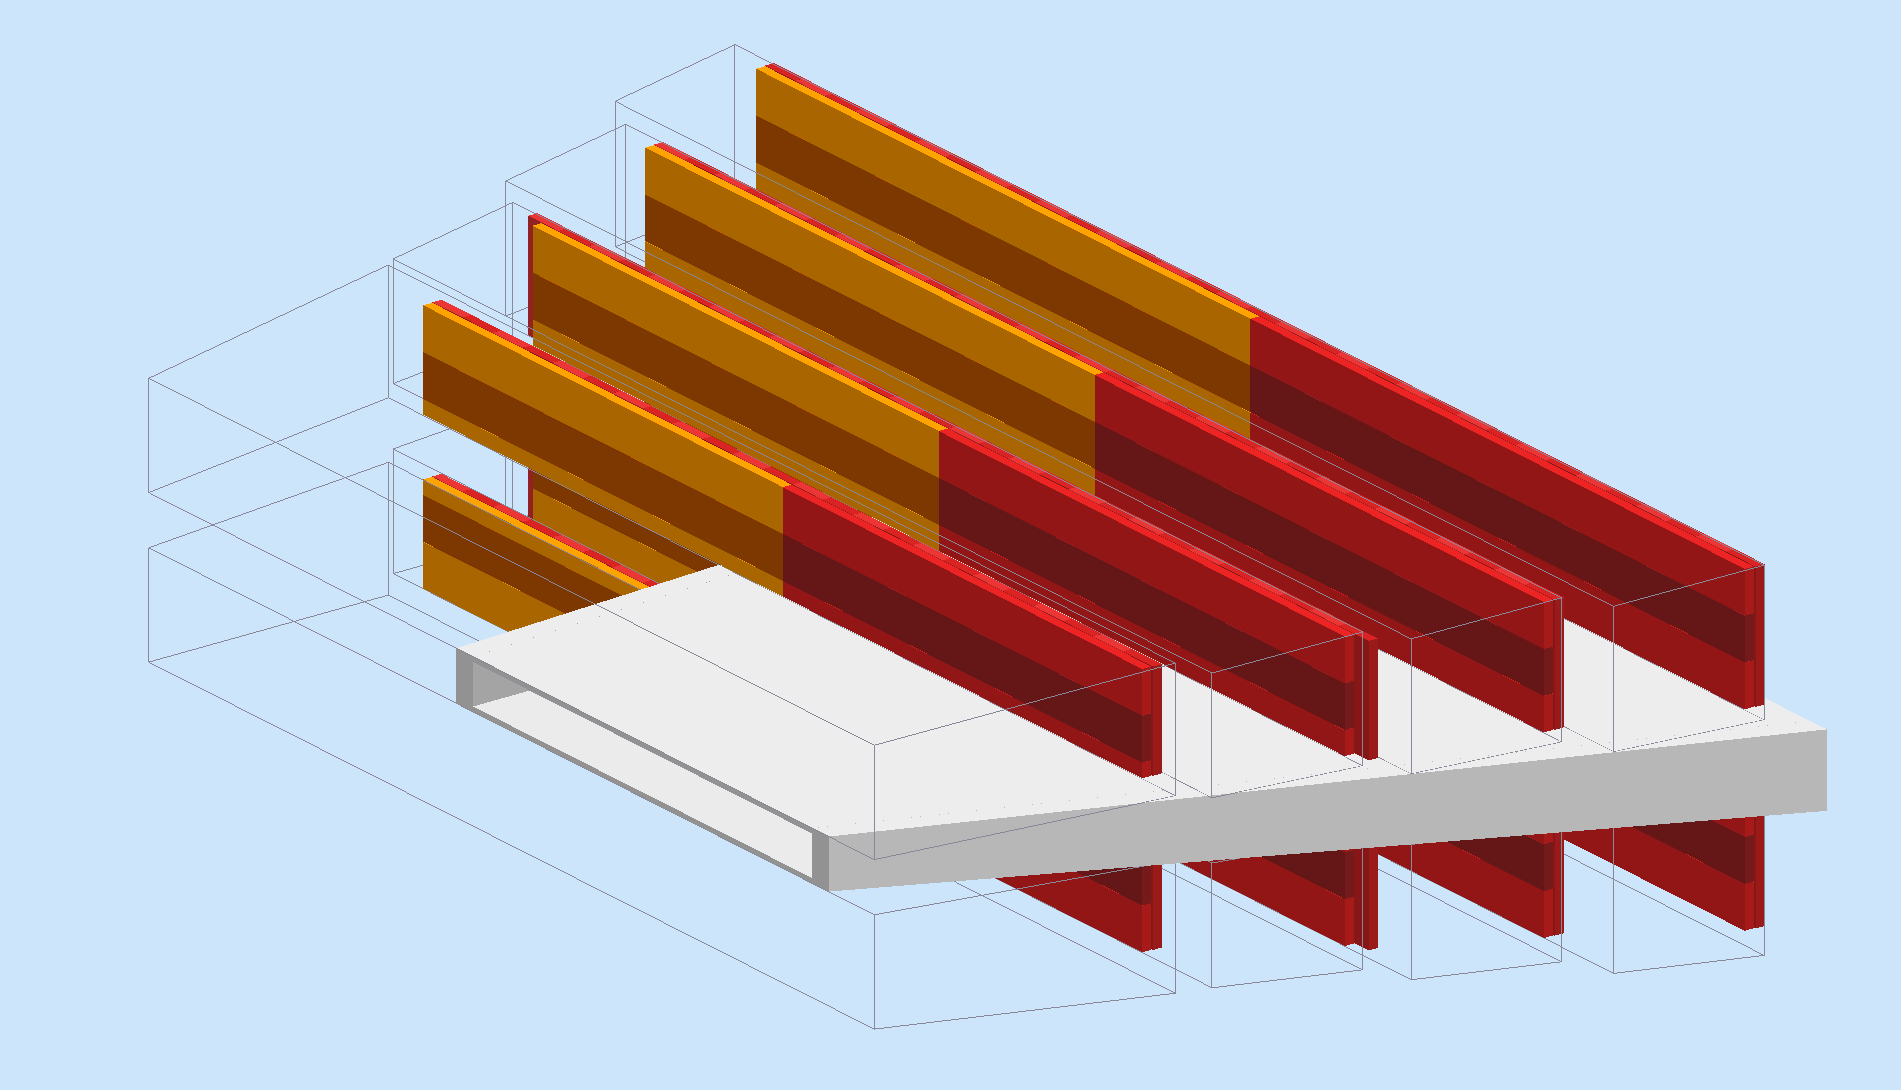
\includegraphics[scale=0.22]{muon/Muon2b.png}
\caption{\small{Horizontal scintillator configuration for the muon counter. Scintillators are
shown in red and yellow/brown.  The white/gray structure is the vacuum box.  Each hodoscope layer (top
and bottom) contains three long strips, read out on both ends.
}}
\label{fig:Muon2p}
\end{figure*}

For the hodoscopes we plan to use the same extruded scintillator strips with embedded wavelength-shifting fiber and multi-anode phototube readout as was developed for the CLAS Preshower Calorimeter. These scintillator strips are 45 mm x 10 mm in cross section, and can be cut to any lengths and widths can be reduced as needed for the muon counter.  Each strip contains two, long tunnels, created in the original extrusion process, into which scintillating fibers can be inserted.  Each hodoscope will consist of one x and one y plane.  In Figure \ref{fig:HPS_view2} in two shades vertical strips of the last hodoscope plane is shown. Figure \ref{fig:Muon2p} in different shades horizontal counters of hodoscope planes are shown. The horizontally aligned strip will extend over the length of the detector and will be read out on each end.  The upper and lower hodoscopes in each plane will have their own vertically aligned strips, which will be read out on only the outer end.  The inner end is inaccessible because of the vacuum box, but there is no particular advantage to having a double readout on these short (135 mm) strips.  

The system can be instrumented with 256 readout channels, in which case the requisite electronics will 
fit into a single VME crate.  Signal from each channel (PMT) 
will be sent to a FADC.  We intend to borrow the CLAS Preshower Calorimeter electronics and HV system.  Similar to ECal, FADCs will be used to construct a muon trigger for the experiment.  In the current design there will be 3 horizontal strips in each of 8 hodoscope planes (24 total) and a total of 208 vertical strips in 8 hodoscope planes.  The number of vertical strips per plane increases slightly with distance from the target to keep a constant angular coverage.  The maximum is 33 per hodoscope in the back plane.

Full Monte Carlo simulations with realistic event rates are currently underway in order to finalize design details of the muon counter.  The crucial issues are the event rates in the scintillators near the beamline (which already has initiated a redesign of the vacuum chamber to reduce background), the target-to-muon-counter tracking resolution and the detection efficiency.  Any changes to the detector as a result are expected to be minor and will not alter the conceptual design presented here.

